% !TeX document-id = {3aec7d78-4a32-4a0f-a5ca-01214b5f7293}
% +---------------------------------------------------------------+
% | Author :    Noémie Plancherel, HEIG-VD
% | Date :      04.03.22
% +---------------------------------------------------------------+

\documentclass[a4paper,11pt,twoside,openright]{book} % Type du document

% compiler avec : pdflatex, bibtex, pdflatex, pdflatex
% !TeX TXS-program:compile = txs:///pdflatex/[--shell-escape]


% +---------------------------------------------------------------+
% | Language
% +---------------------------------------------------------------+
\usepackage[T1]{fontenc}
\usepackage[utf8]{inputenc}
\usepackage[french]{babel}
\usepackage{tablefootnote}
\usepackage{hyperref}
\usepackage{caption}
\newif\ifisconfidential	\isconfidentialfalse

\newif\ifisdraft\isdraftfalse



% +---------------------------------------------------------------+
% | Paramètres
% +---------------------------------------------------------------+

\newcommand{\TBtitle}{Gestionnaires de mots de passe : quelle sécurité ? }
\newcommand{\TBsubtitle}{}%laisser vide si pas de sous-titre
\newcommand{\TByear}{2022}
\newcommand{\TBacademicYears}{2022-2023}

\newcommand{\TBdpt}{Département des Technologie de l'information et de la communication (TIC)}
\newcommand{\TBfiliere}{Filière Télécommunications}
\newcommand{\TBorient}{Orientation Sécurité de l'information}

\newcommand{\TBauthor}{Noémie Plancherel}
\newcommand{\TBsupervisor}{Prof. Sylvain Pasini}

% Confidentiel?
% uncomment if confidential / comment if not confiential
% \isconfidentialtrue

\newcommand{\TBresumePubliable}{
Dans ce travail... Ceci est le résumé publiable...
}

% +---------------------------------------------------------------+



% +-[set path]-------------------------------------+
\usepackage{template/TB-style}
\usepackage{template/TB-macros}
\usepackage{template/TB-template}
%\graphicspath{images/}


\begin{document}

\frontmatter
\pagestyle{empty}

% TITLE and template
% +---------------------------------------------------------------+

\TBmaketitle

\pagestyle{frontmatter}

\TBsecondTitle

\TBpreambule

\TBauthentification


% Cahier des charges
% +---------------------------------------------------------------+
% +---------------------------------------------------------------+
% | Author :    Noémie Plancherel, HEIG-VD
% | Date :      April 1st, 2022
% +---------------------------------------------------------------+


\chapter{Cahier des charges}



\section*{Résumé du problème}
De nos jours, les gestionnaires de mots de passe sont des outils très fréquemment utilisés. En effet, une bonne pratique est d'utiliser un mot de passe par service. De cette manière, si un service est compromis et le mot de passe divulgué, cela n'implique pas les autres. Il est également très important de choisir un mot de passe fort qui ne contient pas d'éléments facilement prévisibles et qui pourrait être brute-forcé rapidement. 

Les gestionnaires de mots de passe permettent principalement de faciliter le stockage des mots de passe qui demandent d'être de plus en plus longs et complexes, de manière à ne pas les réutiliser. Ils permettent également d'ajouter une couche sécuritaire aux mots de passe en les stockant de manière sécurisée et en offrant la possibilité de générer des mots de passe forts.

Ces applications offrent plusieurs fonctionnalités sous la forme de différents types;  elles permettent, entre autres, l'utilisation du cloud afin de stocker les mots de passe sur les serveurs du fournisseur pour faciliter la synchronisation des données entre plusieurs devices (mobile, montre, navigateur, etc.). Certains gestionnaires de mots de passe sont également fréquemment utilisés au sein d'entreprises pour permettre le partage de données. Les entreprises vont généralement utiliser une solution self-hosted où ils auront leur propre infrastructure et stockage. Il existe des extensions de navigateur  qui proposent le remplissage automatique de mots de passe dans les formulaires de connexion. Enfin, il y a également des applications en local qui vont limiter leur utilisation à un seul appareil.

Étant donné que les utilisateurs se reposent grandement sur les gestionnaires de mots de passe, il est important de s'assurer que ces logiciels satisfassent un certain nombre de principes de sécurité ainsi qu'une implémentation robuste afin d'éviter tout vol ou perte de données. 

\section*{Objectifs}
Ce travail de bachelor vise à comprendre les menaces d'un gestionnaire de mots de passe, premièrement de manière générique, puis sur des produits spécifiques, sélectionnés à la suite d'une étude complète, en analysant la sécurité sous différents angles (stockage, mémoire, réseau, cryptographie, etc.). 

Il est réalisé en deux parties distinctes; une première partie qui est une étude approfondie et complète sur les gestionnaires de mots de passe. Elle permet d'analyser les menaces des différents type de gestionnaires de mots de passe et de présenter les exigences sécuritaires qu'il serait nécessaire de garantir. Elle va également se concentrer sur une étude de marché avec une comparaison de plusieurs gestionnaires de mots de passe existants sous différents aspects.

La deuxième partie du travail se concentrera tout d'abord sur la sélection de quelques candidats (environ 4) en fonction de critères établis au préalable. Ensuite, le but est d'évaluer la sécurité de manière complète de chaque gestionnaire de mot de passe sélectionné; chaque élément choisi est analysé et évalué en fonction de différents critères comme les choix cryptographiques utilisés, le stockage, ou encore l'architecture de l'application.

%\begin{enumerate}
%	\item cloud
%	\item local - application desktop
%	\item extension de navigateur
%	\item closed-source
%\end{enumerate}

\subsection*{Livrables}
Les délivrables seront les suivants :
\begin{enumerate}
\item Une documentation contenant :
	\begin{itemize}
	\item Présentation des différents types de gestionnaires de mots de passe
	\item Étude de marché
	\item Une analyse de menaces de différents types de gestionnaires de mots de passe
	\item Spécification des exigences sécuritaires à garantir
	\end{itemize}
\item Analyse sécuritaire des quelques candidats représentatifs (environ 4) :
	\begin{itemize}
	\item Sélection de candidats pour la suite du travail
	\end{itemize}
chaque analyse se décomposera ainsi :
	\begin{itemize}
		\item Sélection de critères d'analyse
		\item Analyse complète de chaque aspect
		\item Rapport des faiblesses trouvées au fabricant
	\end{itemize}
\item Synthèse des résultats
\item Comparaison entre chaque candidat
\end{enumerate}

\subsection*{Déroulement}
En se référant aux dates officielles émises par la HEIG-VD, le travail de bachelor débute le 21 février 2022 et se termine au plus tard le 16 septembre 2022. Il y a 3 dates clés incluant des rendus:
\begin{itemize}
	\item \textbf{16 mai 2022} - rendu du rapport intermédiaire
	\item \textbf{29 juillet 2022} - rendu du rapport final
	\item \textbf{22 août au 16 septembre 2022} - soutenance du travail de bachelor
\end{itemize}

Etant donné, que la soutenance du travail implique l'intervention d'un expert, la date doit être définie entre tous les intervenants.

Le volume du travail de bachelor est de 15 crédit ECTS, soit 450 heures. Le rapport intermédiaire représente 150 heures de travail. Au niveau de la répartition de la charge de travail, cela représente ~13h/semaine jusqu'au 19 juin, puis 45h/semaine jusqu'au rendu, soit le 29 juillet. 



% Planning
% +---------------------------------------------------------------+
% +---------------------------------------------------------------+
% | Author :    Noémie Plancherel, HEIG-VD
% | Date :      April 1st, 2022
% +---------------------------------------------------------------+


\chapter{Planning}
Le travail de bachelor sera séparé en plusieurs tâches et sous-tâches différentes qui permettront de répartir plus facilement le travail sur des périodes de plusieurs semaines. Ci-dessous, le planning détaillé avec toutes les tâches : 

\begin{enumerate}
	\item Préparation
	\begin{itemize}
		\item Rédaction du cahier des charges
		\item Planification
		\item Recherches initiales et introduction
	\end{itemize}
	\item Étude de marché
		\begin{itemize}
			\item Recherche et explication des différents types de gestionnaires de mots de passe
			\item Comparaison des fonctionnalités, du prix et des plateformes disponibles
			\item Analyse du marché actuel et de la demande
			\item Récapitulatif 
		\end{itemize}
	\item Étude sécuritaire
		\begin{itemize}
			\item Présentation de la sécurité implémentée dans les gestionnaires de mots de passe
			\item Identification et analyse des menaces potentielles
			\item Rédaction des exigences sécuritaires
		\end{itemize}
	\item Sélection
		\begin{itemize}
			\item Mise en place des critères de sélection des candidats
			\item Sélection des candidats
		\end{itemize}
	\item Analyse sécuritaire (pour chaque candidat)
		\begin{itemize}
			\item Identification et rédaction des critères d'analyse 
			\item Analyse sécuritaire de chaque aspect
		\end{itemize}
	\item Synthèse (pour chaque candidat)
		\begin{itemize}
			\item Synthèse des résultats
			\item Rapport des faiblesses au fabricant
		\end{itemize}
	\item Synthèse générale
		\begin{itemize}
			\item Comparaison de tous les résultats
			\item Conclusion du travail
		\end{itemize}
	\item Documentation
		\begin{itemize}
			\item Rédaction du rapport
			\item Lecture / visualisation de documents
			\item Tenue d'un journal de travail
		\end{itemize}
\end{enumerate}

Un diagramme de Gantt a également été effectué afin de pouvoir visualiser le planning et ajouter des périodes de temps :
\begin{figure}[h!]
	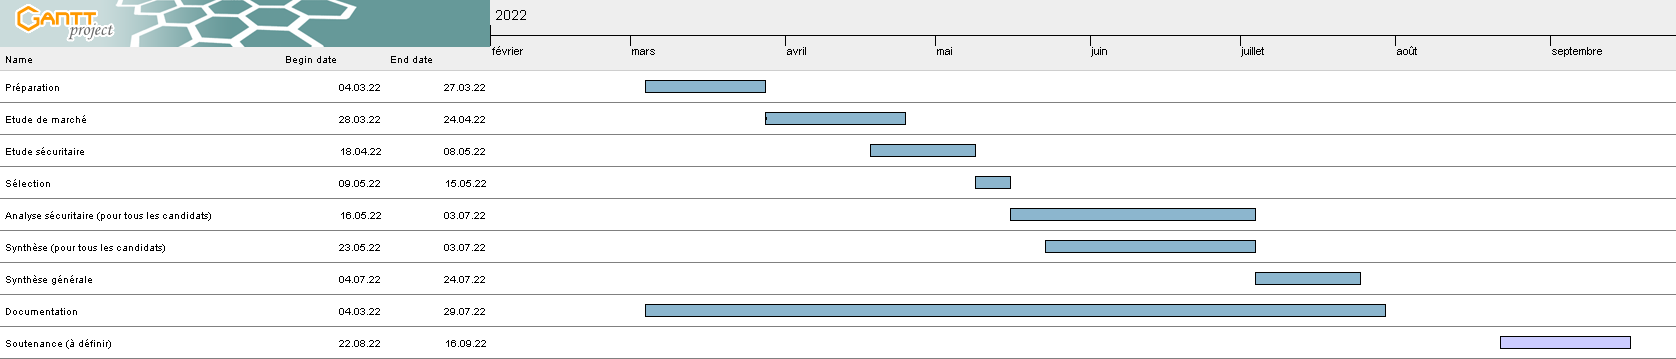
\includegraphics[width=15.5cm]{images/planning.png}
	\caption{Planning du travail de Bachelor}
\end{figure}


% TOC
% +---------------------------------------------------------------+
\tableofcontents
\clearpage


% Content
% +---------------------------------------------------------------+

\mainmatter
\pagestyle{plain}

% +---------------------------------------------------------------+
% | Author :    Noémie Plancherel, HEIG-VD
% | Date :      18.04.2022
% +---------------------------------------------------------------+


\chapter{Introduction}
\label{ch:intro}

Pour un utilisateur lambda, il peut être difficile de se souvenir de tous ses mots de passe tout en s'assurant d'en utiliser un différent pour chaque service afin d'éviter tout vol de données. Typiquement dans ces situations, nous allons naturellement utiliser des mots de passe simples, qui sont facilement mémorisables. Comme, par exemple, utiliser son prénom et sa date de naissance, "123456" ou encore "qwerty". De plus, il est plus simple d'utiliser le même mot de passe pour chacun de ses comptes, afin d'en mémoriser uniquement un seul. 

Cependant, même si l'unique mot de passe qu'on utilise est fort et aléatoire, il n'est pas garanti à 100\% qu'on soit la cible d'aucun attaquant et si une attaque est réalisée, toutes nos données personnelles sont exposées.

Ainsi, dans ce genre de cas, les gestionnaires de mots de passe interviennent et peuvent faciliter le quotidien de la plupart des utilisateurs. 

\section{Fonctionnement général}

Les gestionnaires de mots de passe sont des applications multi-plateformes qui vont permettre de stocker des informations sensibles telles que des mots de passe, numéros de carte de crédit ou encore des fichiers confidentiels. On peut les comparer à des coffres forts.  

Ces derniers proposent un \textit{master password} ou une \textit{master key} qui va permettre d'accéder à l'ensemble des données secrètes. En conséquence, la sécurité repose sur un seul mot de passe principal, ce qui est très bénéfique pour les utilisateurs car ils n'ont qu'un mot de passe à retenir. Une fois l'accès à l'application, l'utilisateur a la possibilité de stocker des données, générer des mots de passe ainsi que se connecter à des services en ligne (remplissage de formulaire d'identification automatique).

Les gestionnaires de mots de passe sont disponibles en plusieurs types différents en fonction du besoin de l'utilisateur et des fonctionnalités proposées. 

\section{Types}

\subsection{Cloud}
Les gestionnaires de mots de passe dans le cloud sont proposés pour un usage personnel ainsi qu'un usage professionnel. Les mots de passe entrés dans le coffre fort vont directement être stockés sur les serveurs du constructeur et ils seront également chiffrés sur ces derniers. Aucun stockage n'est effectué en local.

Le cloud va permettre aux utilisateurs d'avoir accès à leurs données sur n'importe quel device (ordinateur, mobile, montre) et à tout moment. De plus, toutes les données vont être synchronisées sur tous les devices connectés.

À propos de la sécurité, elle repose entièrement sur le provider de l'application car toutes les informations sont stockées sur leurs propres serveurs.

\subsection{Local}
Les applications en local s'installent sur le desktop ou sur le mobile de l'utilisateur. Ces gestionnaires de mots de passe fonctionnent indépendamment et sont offline. Ces produits peuvent donc être utilisés sur une seule machine, par conséquence la synchronisation n'est pas proposée pour ce type de password manager. 

Toutes les données sensibles sont directement stockées et chiffrées sur le device. La sécurité est plutôt bonne comparé à la solution cloud car c'est du hors-ligne, cependant si on récupère / vole le device, la sécurité devient plus faible car il y aurait la possibilité d'avoir accès aux informations sensibles du gestionnaire de mots de passe, via notamment une gestion de mémoire mal gérée. 

Il y a également une solution \textit{on-premise} (ou \textit{self-host}) qui permet d'utiliser sa propre infrastructure locale pour héberger toutes les données du gestionnaire de mots de passe. Les fonctionnalités offertes sont les mêmes que pour les solutions cloud mais le prix est en général plus cher et l'application plus orientée professionnelle.

\subsection{Navigateur}
Le dernier type de gestionnaire de mots de passe sont ceux qui sont basés sur le navigateur (\textit{browser-based}). Les navigateurs les plus populaires, tels que Firefox, Safari ou Chrome offrent ce gestionnaire de mots de passe qui est directement inclu dans ces derniers.
Ils vont faciliter la gestion et la sauvegarde de mots de passe de comptes de sites web. Il y a également la possibilité de synchroniser toutes les données stockées entre tous les devices qui supportent le navigateur en question (Chrome, Firefox, Safari, etc.).

Pour certains navigateurs, les informations sont stockées et chiffrées en local sur le device de l'utilisateur. Si la synchronisation est activée, les données seront également stockées dans le cloud sur les serveurs du constructeur. Un problème de sécurité importante, et la disponibilité des mots de passe sur le navigateur, si aucun master password n'est configuré et qu'on a accès à la machine, les mots de passe sont accessibles en clair sur le navigateur.


% +---------------------------------------------------------------+
% | Author :    Noémie Plancherel, HEIG-VD
% | Date :      18.04.2022
% +---------------------------------------------------------------+



\chapter{Étude de marché}
\label{ch:etude_marche}
Ce chapitre vise à étudier les différentes fonctionnalités offertes par les gestionnaires de mots de passe en les comparant entre plusieurs produits sélectionnés et en établissant un tableau afin d'avoir une meilleure vue d'ensemble.

Nous allons également analyser les différents prix des applications ainsi que présenter où en est le marché actuel afin d'étudier la popularité de ces dernières.

Pour l'étude de marché, les gestionnaires de mots de passe sélectionnés seront: \textit{LastPass}\footnote{\href{https://www.lastpass.com/}{https://www.lastpass.com/}}, \textit{Dashlane}\footnote{\href{https://www.dashlane.com/}{https://www.dashlane.com/}}, \textit{1Password}\footnote{\href{https://1password.com/}{https://1password.com/}}, \textit{KeePass}\footnote{\href{https://keepass.info/}{https://keepass.info/}}, \textit{Bitwarden}\footnote{\href{https://bitwarden.com/}{https://bitwarden.com/}}, \textit{NordPass}\footnote{\href{https://nordpass.com/}{https://nordpass.com/}}, \textit{RoboForm}\footnote{\href{https://www.roboform.com/}{https://www.roboform.com/}}, \textit{Keeper}\footnote{\href{https://www.keepersecurity.com/}{https://www.keepersecurity.com/}}.

Ils ont été sélectionnés en se basant sur leur popularité sur le marché ainsi qu'à la suite de lecture d'articles concernant les meilleurs gestionnaires de mots de passe \cite{BPM22}\cite{gallagher19}\cite{MSPM22}\cite{PM22}.
\section{Fonctionnalités}
Ci-après, une liste des fonctionnalités disponibles dans les gestionnaires de mots de passe. Cette énumération se base sur toutes les fonctionnalités citées sur les websites des différents des \textit{password manager}. \\
\begin{enumerate}
\item Stockage d'informations personnelles (cartes de crédit, passeport, contrats, etc.)
\item Remplissage automatique des formulaires en ligne (auto-complétion)
\item Partage de données entre plusieurs utilisateurs (par exemple, partage d'informations d'identifications entre une famille)
\item Générateur de mots de passe forts
\item Surveillance de la fuite de données ou données compromises
\item Alerte en cas de données compromises
\item Synchronisation de données entre devices (cloud)
\item Authentification à double facteurs
\item Self-hosting
\item Support prioritaire
\item Connexion à l'aide de facteurs biométriques (\textit{fingerprint} ou \textit{facial recognition}) ou d'un pin
\item Possibilité de stockage des secrets en local

\end{enumerate}
Ci-dessous un tableau récapitulatif qui indique quels gestionnaires de mots de passe offre quelles fonctionnalités. 
\begin{longtable}[h]{|c|c|c|c|c|c|c|c|c|c|c|c|c|}
	\hline
	Application & 1 & 2 & 3 & 4 & 5 & 6 & 7 & 8 & 9 & 10 & 11 & 12 \\
	\hline
	LastPass & $\times$ & $\times$ & $\times$! & $\times$* & $\times$* &  $\times$*& $\times$ & $\times$ & & $\times$* & $\times$* & $\times$ \\
		\hline
	Dashlane & $\times$* & $\times$ & $\times$! & $\times$ & $\times$* & $\times$ & $\times$* & $\times$! & & & & $\times$ \\
		\hline
	1Password\footnote{L'application est totalement payante et différents abonnements sont proposés \label{1p}} & $\times$* & $\times$* & $\times$* & $\times$* & & $\times$* & $\times$* & $\times$* & & $\times$* & & $\times$* \\
			\hline
	KeePass \footnote{En général, nécessite l'installation de plugins supplémentaires afin de profiter de toutes les fonctionnalités} & $\times$ & $\times$ &  & $\times$ & $\times$ & & & $\times$ & $\times$ & & $\times$ & $\times$\\
		\hline
	Bitwarden &  & $\times$  & $\times$! & $\times$ & $\times$* & $\times$* & $\times$ & $\times$! & $\times$* &  $\times$* & $\times$!& $\times$ \\
	\hline
	NordPass & $\times$ & $\times$ & $\times$*  & $\times$ & $\times$* & & $\times$ & $\times$ & $\times$* & $\times$* & $\times$ & $\times$\\
	\hline
	RoboForm & $\times$ & $\times$ & $\times$* & $\times$ & & $\times$ & $\times$* & $\times$* & $\times$* & $\times$* & & $\times$\\
	\hline
	Keeper\footnote{Se référer à la note de bas de page \ref{1p}} & $\times$* & $\times$*\footnote{Extension \textit{KeeperFill}} & $\times$* & $\times$* &$\times$* & $\times$* & $\times$* &$\times$* &$\times$* & $\times$* & $\times$* &  $\times$* \\
	\hline
	\caption{Fonctionnalités proposées par les candidats}
\end{longtable} 
$\times$ : L'application propose cette fonctionnalités \\
\textbf{*}\hspace{0.1cm} : Fonctionnalité proposée mais avec un version premium (payante) \\
\textbf{!}\hspace{0.18cm} : Limitations avec une version gratuite \\

Sur tous les candidats sélectionnés, nous remarquons que la plupart offre la majorité des fonctionnalités énumérées plus haut. Nous constatons que l'offre des constructeurs de gestionnaires de mots de passe est assez variée et répond à la demande des particuliers et des entreprises.
\section{Plateformes}
Cette partie va permettre de visualiser sur quelles plateformes les gestionnaires de mots de passe sélectionnés sont supportés. \\
\begin{longtable}[h]{|c|c|c|c|c|c|c|}
	\hline
	Application & Windows & MacOS & Linux & Android & iOS & Navigateur  \\
	\hline
	LastPass & $\times$ & $\times$ & $\times$ & $\times$ & $\times$ &  $\times$\\
		\hline
	Dashlane & $\times$ & $\times$ & $\times$! & $\times$ & $\times$ & $\times$  \\
		\hline
	1Password & $\times$ & $\times$ & $\times$ & $\times$ & $\times$& \\
	\hline
	KeePass & $\times$ & $\times$* & $\times$*  & $\times$* & $\times$* &  $\times$*  \\
		\hline
	Bitwarden & $\times$ & $\times$  & $\times$ & $\times$ & $\times$ & $\times$  \\
		\hline
	NordPass & $\times$ & $\times$ & $\times$  & $\times$ & $\times$ &  \\
		\hline
	RoboForm & $\times$ & $\times$ & $\times$! & $\times$ & & $\times$ \\
		\hline
	Keeper & $\times$ & $\times$ & $\times$ & $\times$ &$\times$ & $\times$ \\
		\hline
	\caption{Plateformes supportées par les différentes applications}
\end{longtable}
$\times$ : L'application est supportée sur ces plateformes \\
\textbf{*}\hspace{0.1cm} :  Des applications (ou des paquets) compatibles avec KeePass Password Safe non-officielles mais contribuées existent \\
\textbf{!}\hspace{0.18cm} : Utilisation via des extensions de navigateur \\

Même si un gestionnaire supporte toutes les plateformes indiquées, il est nécessaire d'aller vérifier les conditions d'utilisation du système, c'est-à-dire les versions des plateformes afin de s'assurer que l'application fonctionnera quand même. 

Cependant, nous constatons que la majorité des applications sont disponibles sur les plateformes les plus courantes, et même si elles ne le sont pas, il y a souvent une solution non-officielle (notamment pour KeePass) ou via le navigateur qui existe.
\section{Prix}
Nous allons passer brièvement en revue les prix proposés par les gestionnaires de mots de passe. Chaque application propose leurs propres gammes de prix avec également des abonnements possibles pour les particuliers, familles ou entreprises. 
\subsection{Particuliers}
Pour la plupart des applications, nous pouvons retrouver 3 gammes de prix; Gratuit, Premium, Famille. L'offre familiale va être plus cher car les gestionnaires de mots de passe sont conçus pour pouvoir avoir plusieurs gestionnaires chiffrés individuels différents. 
Les tarifs ci-dessous sont exprimés en mensualités. \\
\begin{longtable}[h]{|c|c|c|c|}
		\hline
	Application & Gratuit & Premium & Famille \\
		\hline
	LastPass & \$0 & \$3 & \$4  \\
		\hline
	Dashlane & \$0 & \$3.99 & \$5.99 n \\
		\hline
	1Password & non & \$2.99 & \$4.99  \\
		\hline
	KeePass\footnote{gratuit et open-source} & \$0 & non & non   \\
		\hline
	Bitwarden & \$0 & <\$1 & \$3.33   \\
		\hline
	NordPass & \$0 & \$1.84 & \$4.99  \\
	\hline
	RoboForm & \$0 & \$1.99 & \$3.99    \\
	\hline
	Keeper & non & \$2.92 & \$6.25  \\
		\hline
			\caption{2.3 Tarifs pour particuliers}
\end{longtable}
\subsection{Entreprises}
Les entreprises ont quant à elle des prix différents dû à leurs besoins spécifiques où ils pourraient avoir besoin d'un devis personnel afin de choisir l'abonnement qui convient au mieux à leur infrastructure.
\begin{longtable}[h]{|c|c|c|c|}
	\hline
	Application & Gratuit & Premium & Famille \\
	\hline
	LastPass & \$0 & \$3 & \$4  \\
	\hline
	Dashlane & \$0 & \$3.99 & \$5.99 n \\
	\hline
	1Password & non & \$2.99 & \$4.99  \\
	\hline
	KeePass\footnote{gratuit et open-source} & \$0 & non & non   \\
	\hline
	Bitwarden & \$0 & <\$1 & \$3.33   \\
	\hline
	NordPass & \$0 & \$1.84 & \$4.99  \\
	\hline
	RoboForm & \$0 & \$1.99 & \$3.99    \\
	\hline
	Keeper & non & \$2.92 & \$6.25  \\
	\hline
	\caption{2.3 Tarifs pour particuliers}
\end{longtable}
\section{Marché actuel}
prix sur le marché, popularité, lier l'augmentation des cyberattaques avec le covid-19 + peur de perdre ses données
\section{Récapitualtif de l'étude}


% +---------------------------------------------------------------+
% | Author :    Noémie Plancherel, HEIG-VD
% | Date :      18.04.2022
% +---------------------------------------------------------------+

\chapter{Étude sécuritaire}
\label{ch:etude_secu}

Ce chapitre est dédié à toute l'analyse sécuritaire des gestionnaires de mots de passes en général. Nous allons dans un premier temps décrire comment ces applications sont sécurisées en fonction de leur type, puis justifier l'importance d'une forte sécurité suite à l'augmentation de la demande des entreprises et des particuliers.

Dans un second temps, nous allons identifier et analyser toutes les menaces existantes et / ou potentielles des \textit{password manager} en mettant en avant les failles actuellement connues des constructeurs et les conséquences de ces dernières ou des faiblesses qui pourraient survenir à tout moment (par exemple des cyberattaques).

Finalement, nous allons rédiger toutes les exigences sécuritaires que doivent respecter les gestionnaires de mots de passe afin que ces dernières garantissent une utilisation sûre qui évite des pertes ou vol de données.

\section{Implémentation de la sécurité dans les gestionnaires de mots de passe}

Dans cette section, afin de se baser sur des gestionnaires de mots de passe déjà existants et de pouvoir comparer les différentes sécurités implémentées, nous allons reprendre les 8 candidats sélectionnés dans la partie \hyperref[ch:etude_marche]{\textit{étude de marché}}, c'est-à-dire; \textit{LastPass}, \textit{Dashlane}, \textit{1Password}, \textit{KeePass}, \textit{Bitwarden}, \textit{NordPass}, \textit{RoboForm} et \textit{Keeper}. Toutes les informations citées sont basées sur les \textit{security whitepapers} des constructeurs\cite{lastpasssecurity}\cite{dashlanesecurity}\cite{1passwordsecurity}\cite{keepasssecurity}\cite{bitwardensecurity}.

Les gestionnaires de mots de passe sélectionnés fonctionnent tous de la même manière, au final cette méthode est plutôt classique dans les architectures des applications. Un \textit{master password} (qui est seulement connu par l'utilisateur) est généré ou entré par l'utilisateur et va permettre le déverrouillage de l'application et le chiffrement / déchiffrement de toutes les données stockées. 



- utilisation de la mémoire et stockage des secrets
\subsection{Les gestionnaires cloud-based}
\subsection{Les gestionnaires browser-based}
\subsection{Les gestionnaires en local}
\subsection{Partage d'informations}
est-ce que c'est pertinent de parler de ça à ce moment ?
\subsection{Perte du master password}
\subsection{3 états du gestionnaire de mot de passe}

\subsubsection{Etat \textit{Not Running}}
\subsubsection{Etat \textit{Unlocked State}}
en expliquant chaque état et pour l'état unlock expliquer comment est géré le master password, avec des schemas
explication pour extension de navigateur, local et cloud-based
\subsubsection{Etat \textit{Locked State}}

+ facteurs biométriques !

\subsection{Algorithmes cryptographiques}
- les algos utilisés pour le chiffrement et auth des données 
\subsection{L'importance d'une forte sécurité}
\colorbox{pink}{\parbox{15cm}{à voir si utile}}
\section{Analyse des menaces}
\subsection{Failles connues des constructeurs}
\colorbox{pink}{\parbox{15cm}{à voir si je devrais pas les ajouter dans le chapitre de l'analyse de chaque gestionnaire sélectionné}}
\subsection{Conséquences d'une quelconque faiblesse}
\colorbox{pink}{\parbox{15cm}{à voir si utile, mais les conséquences seront sûrement soulignées lorsque je ferai l'analyse de menaces de toute manière}}
\section{Exigences sécuritaires à respecter}

% +---------------------------------------------------------------+
% | Author :    Noémie Plancherel, HEIG-VD
% | Date :      20.09.2022
% +---------------------------------------------------------------+

\chapter{Sélection des candidats}
\label{ch:selection}
Dans ce chapitre, nous allons faire la sélection des gestionnaires de mots de passe que nous analyserons dans le
chapitre suivant. Nous définirons les critères des sélections afin de correctement les choisir, puis nous ferons
notre choix en fonction des candidats sélectionnés. Afin d'avoir une bonne vue d'ensemble sur les fonctionnalités et
la sécurité de chaque application, nous allons reprendre les 9 gestionnaires analysés dans les chapitres précédents.

\section{Critères de sélection}

Cette section va ainsi présenter les critères de sélections pour les candidats avec lesquels on fera une analyse
sécuritaire détaillée.

\textbf{Open-source} - un critère assez important car un gestionnaire de mots de passe open-source pourrait être plus
sûr qu'un gestionnaire closed-source dû au fait qu'importe quel utilisateur peut auditer le code source
indépendamment et peut reporter des failles aux constructeurs. Les applications closed-source comptent à 100\% sur
l'équipe de développement et pourrait faire face à plus d'attaques.

\textbf{Types} - nous allons sélectionner des gestionnaires des 3 types différents afin d'avoir un éventail complet
de gestionnaires de mots de passe existants. Pour faire un rappel, les différents types sont: cloud-based,
local-based et browser-based.

\textbf{Gratuit} - il est bien de prendre en compte ce critère afin d'analyser si un gestionnaire proposant des
fonctionnalités gratuites est plus faible qu'un gestionnaire complètement payant. De plus, il pourrait être
intéressant de comparer la sécurité d'un application qui propose des fonctionnalités gratuites et payantes.

\textbf{Nombre d'utilisateurs} - il est intéressant d'ajouter le critère de la popularité afin de se rendre compte
de l'impact de quelconques vulnérabilités présentes sur l'application et de constater malgré une grande
popularité, s'il y a l'existence de failles non-corrigées ou non-prises en compte.

\textbf{Partage de données} - cette fonctionnalité est assez critique, dû au fait que des données sont partagées
entre plusieurs utilisateurs, il est impératif que les données soient uniquement accessibles par les bonnes personnes
de confiance. Ainsi, il serait intéressant de sélectionner au moins un candidat qui propose cette fonctionnalité pour
évaluer la sécurité.

\textbf{Choix cryptographiques} - ce critère concerne les choix cryptographiques utilisés pour le chiffrement des
données par exemple, ou la dérivation des clés. Il sera important d'évaluer si ces choix sont suffisant. Ainsi, nous
allons sélectionner des candidats qui ont effectuer des choix cryptographiques différents.

\textbf{Plateforme supportée} - l'analyse sécuritaire se fera dans un premier temps sur un ordinateur avec Windows
11, donc les applications doivent être disponibles pour cet OS. La raison pour laquelle nous faisons ce choix est que c'est un des OS les plus populaires sur le marché.

\textbf{Failles connues} - pour quelques gestionnaires de mots de passe, des vulnérabilités ont été découvertes. Pour
certaines, des corrections ont été faites aux applications mais certaines n'ont pas été corrigée malgré un report
vers les constructeurs des gestionnaires. Ainsi, ceci est un aspect important à prendre en compte afin de constater
si les failles ont été corrigées après leurs découvertes.

\section{Choix}
Afin d'avoir une bonne vue d'ensemble sur tous les candidats et de faire une sélection pertinente, nous allons
établir un tableau récapitulatif. Lors du choix, nous allons tenter de couvrir tous les critères proposés avant, afin
de faire une analyse complète et diverse sur tout ce qui existe sur le marché actuellement.

Nous allons donc choisir X candidats pour avoir une bonne vue d'ensemble sur tout ce qui existe.

\begin{figure}[H]
	\centering
	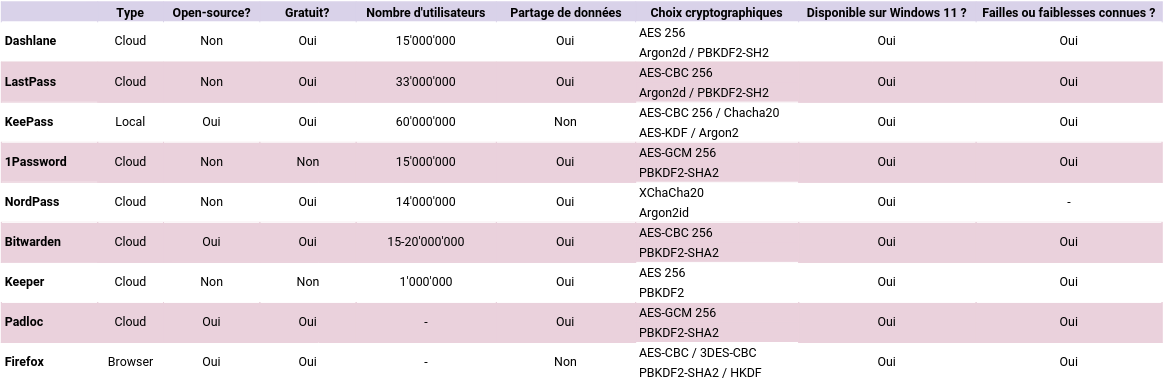
\includegraphics[scale=0.5, angle=90]{images/selection_choix.png}
	\caption{Comparatif des candidats pour la sélection}
\end{figure}

Ainsi, nous allons sélectionner:
\begin{itemize}
	\item LastPass
	\item KeePass
	\item Firefox
	\item 1Password
\end{itemize}

Chaque chapitre dédié aux gestionnaires de mots de passe sélectionnés se basera sur les exigences sécuritaires que nous avons définis au chapitre précédent et sur les vulnérabilités et faiblesses déjà connues. 

À chaque début de chapitre, nous établirons les critères d'évaluation de la sécurité de l'application. Les critères seront à chaque fois différents en fonction du type ou des fonctionnalités proposées. 




% +---------------------------------------------------------------+
% | Author :    Sylvain Pasini, HEIG-VD
% | Date :       June 3rd, 2021
% +---------------------------------------------------------------+


\chapter{Conclusion}



% +---------------------------------------------------------------+
%\backmatter

\cleardoublepage
\phantomsection
\addcontentsline{toc}{chapter}{Bibliographie}
\bibliographystyle{plain}
\bibliography{chapters/biblio}
\nocite{*} %ajoute tout ce qu'il y a dans le bibtex

\cleardoublepage
\phantomsection
\addcontentsline{toc}{chapter}{Liste des figures}
\listoffigures

\cleardoublepage
\phantomsection
\addcontentsline{toc}{chapter}{Liste des tableaux}
\listoftables

\cleardoublepage
\phantomsection
\addcontentsline{toc}{chapter}{Liste des listings}
%\listoflistings
\tcblistof[{\chapter*}]{mypyg}{Liste des listings}


% Annexes
% +---------------------------------------------------------------+
\appendix

% +---------------------------------------------------------------+
% | Author :    Sylvain Pasini, HEIG-VD
% | Date :       June 3rd, 2021
% +---------------------------------------------------------------+


\chapter{Outils utilisés pour la compilation}

%exemple
\lipsum[5-6]


% +---------------------------------------------------------------+
% | Author :    Sylvain Pasini, HEIG-VD
% | Date :       June 3rd, 2021
% +---------------------------------------------------------------+


\chapter{Journal de travail}

\begin{landscape}

\begin{longtable}[c]{lp{10cm}rrrr}
    \caption{Journal de travail}\\

    \hline
    Date & Description & Rech. [h] & Dev. [h] & Rapport [h] & Admin [h] \\
    \hline
    \endfirsthead
    
    \hline
    Date & Description & Rech. [h] & Dev. [h] & Rapport [h] & Admin [h] \\
    \hline
    \endhead
    
    \multicolumn{6}{r}{\small \it Le journal de travail continue à la page suivante.} \\
    \normalsize
    \endfoot
    
    \hline
    \endlastfoot


  % Work
    > 20.09.22
    & Discussion avec le professeur responsable, établissement du cahier des charges, introduction
    & 7 %recherche
    & 0 %dev
    & 10 %reporting
    & 4\\ %admin
    
	20.09.2022 
	& Update + organisation du TB, planing, relire le début du TB déjà commencé, avancement de l’étude du marché (fonctionnalités, plateformes, prix), lecture d’articles
	& 2 %recherche
	& 0 %dev
	& 5 %reporting
	& 1\\ %admin

	21.09.2022 
	& Recherches sur les statistiques des gestionnaires de mots de passe sur le marché, rédaction du chapitre étude de marché (terminé ce jour-ci)
	& 3 %recherche
	& 0 %dev
	& 3 %reporting
	& 0\\ %admin

	22.09.2022
	& Introduction et organisation du chapitre étude sécuritaire, recherche et lecture sur les différentes implémentations sécuritaire des gestionnaires de mots de passe
	& 3 %recherche
	& 0 %dev
	& 1 %reporting
	& 1\\ %admin

	23.09.2022 
	& Recherche et lecture sur les différentes implémentations sécuritaire des gestionnaires de mots de passe et organisation du rapport
	& 1 %recherche
	& 0 %dev
	& 1 %reporting
	& 0\\ %admin

	26.09.2022  
	& Recherche et lecture sur les gestionnaires de mots de passe browser-based, rédaction dans le rapport à ce propos
	& 4 %recherche
	& 0 %dev
	& 1 %reporting
	& 0\\ %admin
	
	
	27.09.2022  
	& Recherche et lecture sur les gestionnaires de mots de passe browser-based et local-based, et rédaction dans le rapport
	& 3 %recherche
	& 0 %dev
	& 2 %reporting
	& 0\\ %admin
	
	28.09.2022  
	& Recherche et lecture sur les gestionnaires de mots de passe browser-based et local-based, et rédaction dans le rapport
	& 4 %recherche
	& 0 %dev
	& 1 %reporting
	& 0\\ %admin

	29.09.2022  
	& Recherche et lecture sur les gestionnaires de mots de passe local-based, et rédaction dans le rapport
	& 5 %recherche
	& 0 %dev
	& 3 %reporting
	& 0\\ %admin

	30.09.2022 
	& Rédaction de la section du partage d'informations, des 3 états du gestionnaires de mots de passe 
	& 1 %recherche
	& 0 %dev
	& 4 %reporting
	& 0\\ %admin

	03.10.2022 
	& Fin du chapitre 3 sur analyse de menaces, lecture sur la modélisation de menaces et la norme que je souhaite suivre
	& 7 %recherche
	& 0 %dev
	& 1 %reporting
	& 0\\ %admin

	04.10.2022
	& Début chapitre analyse de menaces et lecture de la norme choisie
	& 6 %recherche
	& 0 %dev
	& 2 %reporting
	& 0\\ %admin
	
	05.10.2022
	& Lecture et rédaction établissement du contexte de l'analyse de menaces
	& 5 %recherche
	& 0 %dev
	& 3 %reporting
	& 0\\ %admin

	06.10.2022 
	& Lecture et rédaction établissement du contexte de l'analyse de menaces
	& 2 %recherche
	& 0 %dev
	& 6 %reporting
	& 0\\ %admin

	07.10.2022 
	& Lecture et rédaction identification des risques de l'analyse de menaces
	& 5 %recherche
	& 0 %dev
	& 3 %reporting
	& 0\\ %admin

	09.10.20220 
	& Lecture et rédaction identification des risques de l'analyse de menaces
	& 2 %recherche
	& 0 %dev
	& 2 %reporting
	& 0\\ %admin
	
	10.10.20220 
	& Lecture et rédaction identification des risques de l'analyse de menaces
	& 3 %recherche
	& 0 %dev
	& 5 %reporting
	& 0\\ %admin
	
	11.10.20220 
	& Rédaction et lecture analyses des risques et évaluation des risques
	& 4 %recherche
	& 0 %dev
	& 4 %reporting
	& 0\\ %admin
	
	12.10.20220 
	& Rédaction et lecture analyses des risques et évaluation des risques
	& 3 %recherche
	& 0 %dev
	& 4 %reporting
	& 0\\ %admin
	
	13.10.20220 
	& Rédaction du traitement des risques et lecture à ce propos avec les contremesures possibles
	& 3 %recherche
	& 0 %dev
	& 3 %reporting
	& 0\\ %admin
	
	14.10.20220 
	& Rédaction de la section exigences sécuritaires à respecter, relecture du TB, organisation du rapport et rendu intermédiaire du rapport
	& 1 %recherche
	& 0 %dev
	& 6 %reporting
	& 0\\ %admin

	16.10.20220
	& Rédaction de la sélection des candidats
	& 2 %recherche
	& 0 %dev
	& 6 %reporting
	& 0\\ %admin
	
\end{longtable}


\end{landscape}


\end{document}

% Auteur : Sylvain Pasini, HEIG-VD, 2021
